\section{Graphs}

\frame{
{Part 1: Graph Definitions}

\tableofcontents[currentsection,hideallsubsections, firstsection=1, sections={1-3}]
}

\subsection{Motivations}

\begin{frame}{Using Graphs to Solve Problems}{First Example Problem: Course Registration}

  We can represent a list of courses in a university, and their requirements, using a graph structure. For example, to take \emph{"Computer Graphics"}, you need to take \emph{"Programming Theory"} and \emph{"Linear Algebra"} first.\medskip

  If you take two lectures per semester, how long would it take you to graduate? Why?

  \begin{tabular}{p{.1\textwidth}|p{.45\textwidth}||p{.3\textwidth}}
    \hline
    Code & Lecture & Prerequisites \\
    \hline
    0000 & {\small Social Questions} & \emph{none} \\
    0001 & {\small Intro to Programming} & \emph{none} \\
    0002 & {\small Calculus I} & \emph{none} \\
    0003 & {\small Programming Theory} & \emph{0001} \\
    0004 & {\small Linear Algebra} & \emph{0000, 0002} \\
    0005 & {\small Programming Challenges} & \emph{0000, 0001, 0003} \\
    0006 & {\small Computer Graphics} & \emph{0003, 0004} \\
    \hline
  \end{tabular}
\end{frame}


\begin{frame}{Using Graphs to Solve Problems}{First Example Problem: Course Registration}

  The university proposes a new lecture, \emph{"Maths for Computer Science"}. The updated table is below. \medskip

  How long does it take to graduate now? Why?

  \begin{tabular}{p{.1\textwidth}|p{.45\textwidth}||p{.3\textwidth}}
    \hline
    Code & Lecture & Prerequisites \\
    \hline
    0000 & {\small Social Questions} & \emph{none} \\
    0001 & {\small Intro to Programming} & \emph{none} \\
    0002 & {\small Calculus I} & \emph{none} \\
    0003 & {\small Programming Theory} & \emph{0001, {\bf 0007}} \\
    0004 & {\small Linear Algebra} & \emph{0000, 0002} \\
    0005 & {\small Programming Challenges} & \emph{0000, 0001, 0003} \\
    0006 & {\small Computer Graphics} & \emph{0003, 0004} \\
    {\bf 0007} & {\small {\bf Maths for Computer Science}} & {\bf\emph{0005}} \\
    \hline
  \end{tabular}
\end{frame}

\begin{frame}{Using Graphs to Solve Problems}{Second Example Problem: Airplane}
  \begin{columns}

    \column{0.3\textwidth}
    In an airport, each airplane needs a gate when it is on the ground.\medskip

    If we know the landing and departing time of each plane, what is the minimum number of gates necessary?
    \column{0.7\textwidth}
    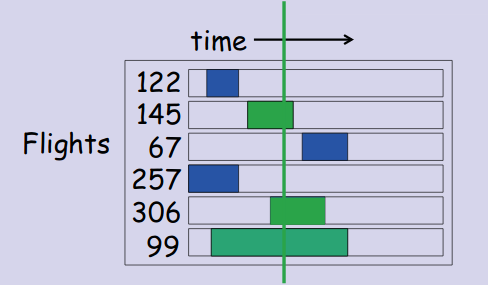
\includegraphics[width=\textwidth]{../img/gatetable}
  \end{columns}
\end{frame}

\begin{frame}[t]{Problems as Graphs}
  Many problems that can be described by the \emph{relationship} between entities in the problem can be represented as graphs.\bigskip

  \begin{itemize}
    \item A course is a prerequisite to another one;
    \item Two planes are landed at the same time;
    \item Webpages and the links between them;
  \end{itemize}\bigskip

  These relationships can be described mathematically using a graph structure.

  \vfill 

  \begin{block}{}
  Graph representation allows us to use the same mathematical tools for different problems!
  \end{block}
\end{frame}

\subsection{Definitions}

\begin{frame}[t]{Graph Basic Definitions}

    \begin{columns}
      \column{0.4\textwidth}
      \begin{center}
        \begin{tikzpicture}[scale=.8,auto,swap]
  \tikzset{edge/.style = {->,>=latex'}}
  \node[vertex] (a) at (0,0) {a};
  \node[vertex] (b) at (2,3) {b};
  \node[vertex] (c) at (4,2) {c};
    \node[vertex] (d) at (4,0) {d};
    \draw[edge] (a) to (b);
    \draw[edge] (a) to (c);
    \draw[edge] (c) to (b);
    \draw[edge] (d) to (c);
    \draw[edge] (d) to (a);
\end{tikzpicture}

      \end{center}

      \column{0.6\textwidth}
        A {\bf graph} $G$ is defined by a set of vertices $V$, and a set of edges $E$.\bigskip

        \begin{itemize}
          \item $G = (V,E)$
          \item $V = \{a,b,c,d\}$
          \item $E = \{(a,b), (a,c), (c,b), (d,c), (d,a)\}$
        \end{itemize}\bigskip

         A {\bf directed graph (digraph)} is a graph where each edge has a {\bf direction}.\medskip

         An {\bf undirected graph} is a graph where the edges do not have a direction ($(a,b) \iff (b,a)$).
    \end{columns}
\end{frame}

\begin{frame}{Graphs and Relations}{Remember Lecture 2?}

  \begin{columns}
    \column{0.4\textwidth}
    \begin{center}
      \begin{tikzpicture}[scale=3,auto,swap]
      \tikzset{edge/.style = {->,>=latex'}}
      \node[vertex] (a) at (0,1) {a};
      \node[vertex] (b) at (1,1) {b};
      \node[vertex] (c) at (1,0) {c};
      \node[vertex] (d) at (0,0) {d};
      \draw[edge] (a) to (c);
      \draw[edge] (a) to (b);
      \draw[edge] (c) to (b);
      \end{tikzpicture}
    \end{center}
    \column{0.6\textwidth}

    Graph $G = (V, E)$
    \begin{itemize}
      \item Set of vertices $V = \{a,b,c,d\}$
      \item Set of edges $E = \{(a,c),(a,b),(c,b)\}$
    \end{itemize}\bigskip

    \begin{itemize}
    \item Every graph can be described as \structure{a binary relation $V \to V$}
    \begin{itemize}
      \item $E(a) = \{b,c\}$
      \item $E(c) = \{b\}$
      \item $E(d) = \emptyset$
    \end{itemize}
    
    \bigskip

    \item And every binary relation can be described as a directed graph too!
    \end{itemize}
  \end{columns}
\end{frame}

\begin{frame}{Matrix Representation of a Digraph}

  \begin{columns}
    \column{0.5\textwidth}
    \begin{center}
    \begin{tikzpicture}[scale=1.5,auto,swap]
      \tikzset{edge/.style = {->,>=latex'}}
      \node[vertex] (a) at (0,1) {a};
      \node[vertex] (b) at (0,0) {b};
      \node[vertex] (c) at (0,-1) {c};
      \node[vertex] (d) at (2,0) {d};
      \node[vertex] (e) at (3,1) {e};
      \node[vertex] (f) at (3,-1) {f};
      \draw[edge] (a) to (b);
      \draw[edge] (c) to (b);
      \draw[edge] (b) to (d);
      \draw[edge] (d) to (a);
      \draw[edge] (c) to (d);
      \draw[edge] (d) to (e);
      \draw[edge] (e) to (f);
      \draw[edge] (f) to (d);
    \end{tikzpicture}
  \end{center}

    \column{0.5\textwidth}

    {\larger
      \begin{tabular}{c|cccccc}
        & a & b & c & d & e & f \\
        \hline
        a &0&1&0&0&0&0\\
        b &0&0&0&1&0&0\\
        c &0&1&0&1&0&0\\
        d &1&0&0&0&1&0\\
        e &0&0&0&0&0&1\\
        f &0&0&0&1&0&0\\
      \end{tabular}
    }
  \end{columns}\bigskip

  \begin{itemize}
    \item A digraph is represented by a $|V|x|V|$ binary matrix ({\bf adjacency matrix})
    \item If there is an edge between $v_i$ and $v_j$, then $A_{i,j} = 1$, else $A_{i,j} = 0$ 
    \item Another way to state it:    $A(v_i,v_j) = 1 \iff v_j \in E(v_i)$
  \end{itemize}
\end{frame}
